\chapter{Introduction}

During the last years the interest of robotic science and the development of
robots increase enormous. Reasons for that are, the unstoppable technological
progress of hard and software techniques, but also the necessity to replace
humans with machines in dangerous, monotonous or unreachable industrial
environments (medical, space, aviation and so far). One area of these interests
is the aerial platform and the realization of \UAV, which are mostly controlled
via remote control or fly autonomous. These aircraft vehicles have several
capabilities like in military or rescue operations with special environments like
a burning house. For such indoor operation it is important to
focus, that some kind of feedback sensors like GPS-sensors could not work
satisfactory. In such cases \UAV s faces problems with the self stabilization,
because their physical behaviour is in generally unstable 
\citebib[p.1 Introduction]{BloWeiScaSie10}. Most of the approaches to stabilize
\UAV work with a clever combination of sensor equipment and control algorithms.
Mostly this controller uses a \IMU which is mounted on board and includes
accelerations sensors to detect movements in the given \DOF. Actual acceleration
sensors, which are used for this purpose, are \MEMS or fiberoptic sensors which
have a finite precision and unacceptable error propagation in case of integration
for velocity or position detection 
\citebib[p.p.11-13 Function Principles of MEMS, Sources of Error]{Fac08}.
\newpage
 This problem also is a field of research at the Quadrocopter project of the
 \HSE \citebib[Website]{HSE10}.

\begin{figure}[!htbp]
	\centering
		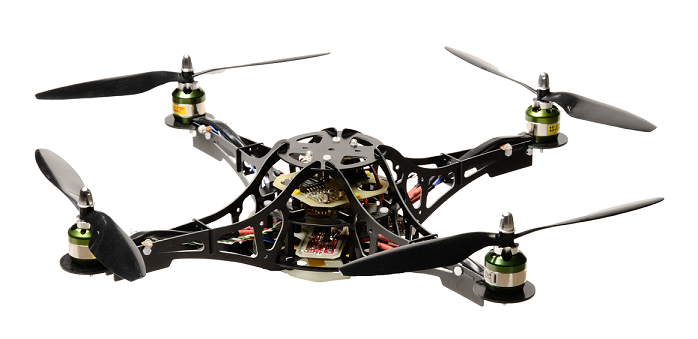
\includegraphics[width=0.75\textwidth]{graphic/QuadrocopterImage.png}
	\caption{HSE Quadrocopter}
	\label{fig:QuadrocopterImage}
\end{figure}


\section{Project State}

The quadrocopter project of the \HSE was launched with the goal to build a
system from the scratch, which is developed by students, scientific workers and
Professors. In a first project the Printed Circuit Board which hosts
the parts necessary to control the quadrocopter was designed by students at the
faculty of Mechatronics and Electrical Engineering in Goeppingen. This project
groups' focus was then on the simulation, implementation of the basic functions
and visualization of the actual condition of the aircraft. The first two project
groups already show the benefit of this project, a multidisciplinary development
including hardware design, application development, embedded programming,
simulation and the interfaces between these special fields. In the year
2009, the Faculty of Information technology adopted the development of the
project with the aim to solve problems which came up in the previous development
and to redesign the soft- and hardware architecture.
\newpage So a new hardware design was
developed in a corporation between the two faculties with the outcome of a \CCU
which can detect inertial movements in six \DOF and can control the four
actuators of the quadrocopter via so called brushless controllers.
One of the biggest unresolved problems since yet is the development of a robust
controller and the elimination of drifts which especially come up at the hovering state.
 The practice and the experience of previous developments show, that it is
indispensable to proof new developments with a simulation before they will be
realized at the real \UAV. So the main topic and the focus of this Master�s
Thesis will be on the development of a simulation which shows potential solutions
of the mentioned problems and the research and evaluation of the outcome results.

%\section{Motivation and Novel Aspect}
